\chapter{Evaluation}

%\section{Experimental Setup}
\section{The Guided Transcoding Chain}
Our test environment for running \gls{gt} simulations has many components. A full simulation chain entails several encodings at multiple \gls{qp} values, decoding and downscaling each encoding to a number of different sizes, re-encoding, generating \gls{si} and reconstructing the sequences. Additionally, we want to measure bit rate and \gls{psnr} at several points in the simulation, and be able to access all the data in a structured manner to try to make sense of it and to compare different simulations.

We wrote a test environment in Python that allows us to easily specify sets of \gls{qp} values and downscaled sizes, together with \gls{gt} schemes; pruning, partial pruning or deflation, and options like \gls{sbh} and \gls{rdoq}.

\subsection{Encoding the Original}
The pruning and deflation scenarios differ in the way side-information is generated but many parts of the chain works the same way, using most of the same programs. We first describe the \gls{gt} approach common to both methods and then elaborate on the details of each case.

The first step is always to encode the original test sequences. Our suite uses five \gls{hevc} sequences that belong to the \gls{jvt} common test conditions, class B: Kimono, ParkScene, Cactus, BasketballDrive and BQTerrace. Still frames can be seen in \cref{fig:test-sequences}. They represent a wide variety of possible use-cases for video encoding: varying degrees of movement, static camera and panning movements, and frame rates varying from 24 to 60 \gls{fps}. All sequences have a bit depth of 8 bits and $1920 \times 1080$ resolution~\cite{Wien_Coding_Tools}. Each clip is ten seconds long, giving frame count between 240 and 600 which \gls{jvt} considers sufficient to get a qualified assessment of video quality, while still keeping the required encoding complexity sufficiently low~\cite{Wien_Coding_Tools}.

Some of our sequences have a copyright frame as the last one, giving a total of 601 frames for a 60 \gls{fps} video. This frame frame is not expected to used in simulations, and we exclude it from all of our encodings and references, and it should therefor have no effect on our results.

\begin{figure}[!tbp]
  \centering
  \begin{minipage}[b]{0.4\textwidth}
    
\includegraphics[scale=0.1]{pictures/yuv-player-captures/BQTerrace_1920x1080_60_1}
  \end{minipage}
  \hfill
  \begin{minipage}[b]{0.4\textwidth}
    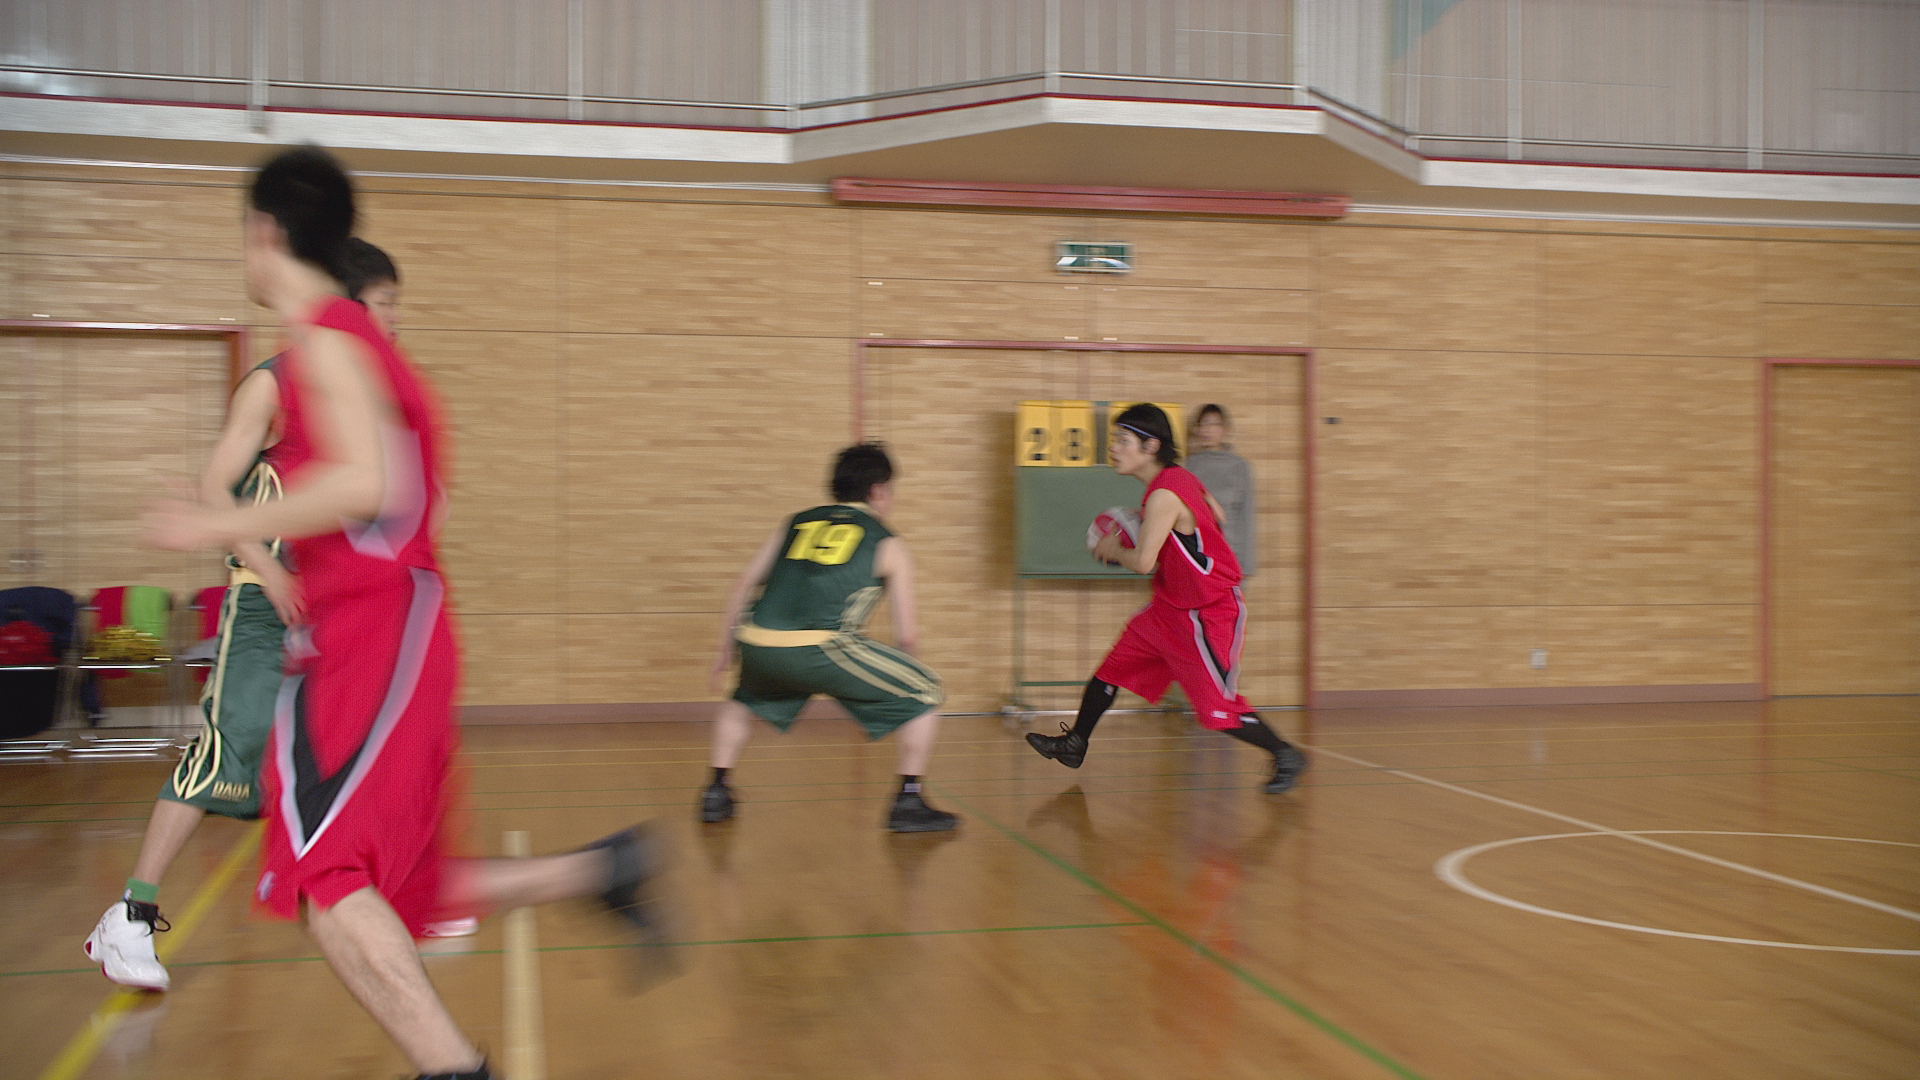
\includegraphics[scale=0.1]{pictures/yuv-player-captures/BasketballDrive_1920x1080_50_1}
  \end{minipage}
  \caption{Still frames from our HEVC standard sequences}
  \label{fig:test-sequences}
\end{figure}

All the videos we work with are stored in progressive scan, meaning simply that each individual frame contains information about all of its own pixels, as opposed to interlaced scan where a frame is split over two successive frames, each one holding half. We will follow the convention regarding scan modes and refer our resolutions as 1080p, 720p, etc., thus omitting the frame width.

For each original video we create four encoding with \gls{qp} values 22, 26, 30 and 34, and refer to these as $QP_{base}$. All encoding and later re-encoding are performed using the \gls{hm} encoder with a configuration file specifying \textit{\gls{hevc} Main profile} and the \textit{randomaccess} \gls{gop} structure~\cite{Wien_Coding_Tools}. Randomaccess has a GOP size of 8 and coding order 0-8-4-2-1-3-6-5-7, after which it skips to frame 16, repeats the same pattern, and then continues like that for the whole sequence~\cite{Wien_Coding_Tools}.

All of the outputs from the initial encoding step are referred to as \gls{hq} bitstreams. Generating these is by far the most expensive part of any simulation in terms of computational complexity, taking around 15 hours on our cluster environment (see \cref{subsec:cluster}), so we make sure to store them and always try to re-use bitstreams for any simulation where all the applicable test parameters are the same.

\subsection{Re-Encoding and Pruning}
\label{subsec:re-encoding}
For the pruning scenario, the next step is to decode the \gls{hq} bitstreams and downscale from 1080p to 720p, 540p and 360p representations which we refer to as the \gls{lq} resolutions. Our downscaler only supports downscaling to 1/2 or 2/3 size, so to generate a 360p video from 1080p we always have to get there via an intermediate 720p step.

We re-encode with the same $QP$ value and with $QP + 2$. That is, for an \gls{hq} bitstream generated with $QP=22$ we create re-encodings with \gls{qp} values 22 and 24, for \gls{hq} bitstreams generated with $QP=26$ we use 26 and 28, and so on. This gives us a wide array of test cases to accurately quantify the effect on \gls{qp} value on video quality, bit rate and reconstruction time.

After re-encoding, we prune the \gls{lq} bitsteams to generate \gls{si}. We either do partial or full pruning, the difference at this stage is just an input parameter. In an real real-world application we would then store the \gls{si} instead of the \gls{lq} bitsteam, saving a certain amount of storage space. Of course, for the sake of the simulation, we keep both. We sometimes refer to the \gls{si} and the bitstreams as \textit{uplink data}.

We also downscale the original sequences to the \gls{lq} resolutions for use as reference data when calculating \gls{psnr}, and then encode them to act as \gls{lq} bitstreams in the deflation scenario. For this we use all applicable \gls{qp} values; 22, 24, 26, 28, 30, 32, 34 and 36, which we refer to as $QP_{extended}$.

\subsection{Regenerating Sequences}
The HQ bitstreams together with the \gls{si} is used to reconstruct videos. For each test case, we reconstruct the video to make sure everything works as expected, then measure bit rate and \gls{psnr} again. This is not strictly necessary because by definition the reconstructions are perfect, so we could just as well have re-used the data for the corresponding \gls{lq} bitstream. But this acts as a good sanity check for the simulation.


%\section{Evaluation Environment}
\section{Cluster Simulations}
\label{subsec:cluster}
For any simulation of five tests sequences, four \gls{qp} values, three \gls{lq} resolutions and two additional \gls{qp} values, we get a total of $5 \times 4 \times 3 \times2 = 120$ test cases.

Each combination is submitted to a cluster system as a self-contained \textit{job}. The cluster allows for faster calculations than running locally, and allows hundreds of jobs to run in parallel without affecting performance. The cluster is shared among many users and a has its own scheduler. One job will for example correspond to BasketballDrive, \gls{qp} 22, 540p and \gls{qp} 24, and will then only be concerned with the creation of the specific files needed for that test case.

A separate meta-script is responsible for iterating over simulation parameters and starting each of the 120 jobs that make up one simulation. Jobs will then work in parallel, sharing many of the same files, and together generate every combination of files needed to evaluate a full simulation. This script also creates a test{\_}data file to keep track of the locations of all data files holding bit rate and \gls{psnr} information.

To allow jobs to work in parallel and read and write from the same directory structure without destroying data, we implemented a locking system. Because cluster jobs cannot directly communicate with each other we could not utilize traditional threading. So we represented locks as empty files named as the target file plus the extra file extension ".lock", it is then up to each script to respect the lock. All the jobs share the same storage area, but also have private tmp areas where files are created. Whenever a job wants to create a file, it attempts to lock it in the storage area. If the lock creation fails because the lock file already exists then we assume that some other job is busy creating that file, and we enter a sleep loop that regularly checks the existence of the lock and only exists when the lock has been removed, at which point our desired file must exist in the storage area.

The execution works as follows; if two jobs both have parameters BasketballDrive and \gls{qp} 22, but one has \gls{lq} resolution 720p and the other 540p, then both will want to create an \gls{hq} bitstream of BasketballDrive with \gls{qp} 22. Assuming that this file does not already exist from a previous simulation -- if it does then both scripts move on the their next step -- both jobs will try to acquire the lock but only one will succeed. The job that grabs the lock starts creating the bitstream in its tmp area while the other jobs sleeps. After the file has been created, the job moves the file over to the public storage area and then removes the lock. This way, no in-progress or incomplete files will ever exist in the storage area, and furthermore we won't have to worry about race conditions in the code. If the file is not locked -- and it exists in the storage area -- it is guaranteed to be complete.

Especially early on in a simulation chain, many jobs will share the same files. Only the \gls{lq} encoding is actually unique to a specific job. For example, out of 120 jobs, evenly divided groups of 24 jobs each share the exact same \gls{hq} bitstream file.

Every file in the simulation chain follows the same pattern of creation; the job checks for the existence of the file in the storage area and whenever it find it there, it swiftly moves on to the next step. If all files are already created, the jobs runs through the whole chain without actually creating any files and then exits cleanly. This structure allows for maximum file reuse whenever we want to test new simulation parameters. If we run a simulation where a parameter that only affects the latter part our chain has been changed, the jobs will find many of its files already present and won't have to spend any to recreate them. In many simulations we thus can avoid the encoding the \gls{hq} bitstreams, for example, cutting down the total simulation time by many hours.

\begin{figure}
\dirtree{%
        .1 Cactus{\_}1920x1080{\_}50.
        .2 sbh0{\_}rdoq0.
        .3 qp22.
        .4 hq{\_}bit{\_}1920x1080{\_}50.bin.
        .4 hq{\_}bit{\_}1920x1080{\_}50{\_}dec.yuv.
        .4 hq{\_}bitstream{\_}data.txt.
        .4 540p.
        .5 ds{\_}960x540{\_}50.yuv.
        .5 qp22.
        .6 downscaled{\_}original{\_}data.txt.
        .6 ds{\_}org{\_}960x540{\_}50.bin.
        .6 ds{\_}org{\_}960x540{\_}50{\_}dec.yuv.
        .6 deflation.
        .7 def{\_}960x540{\_}50.bin.
        .7 def{\_}960x540{\_}50{\_}dec.yuv.
        .7 deflation{\_}data.txt.
        .7 inf{\_}960x540{\_}50.bin.
        .7 inf{\_}960x540{\_}50{\_}dec.yuv.
        .7 inflation{\_}data.txt.
        .6 pruning.
        .7 reenc{\_}960x540{\_}50.bin.
        .7 reenc{\_}960x540{\_}50{\_}dec.yuv.
        .7 full{\_}pruning.
        .8 reconstruction{\_}time.txt.
        .8 pruned{\_}960x540{\_}50.bin.
        .8 pruned{\_}data.txt.
        .8 pruned{\_}960x540{\_}50{\_}dec.yuv.
        .8 recon{\_}960x540{\_}50.bin.
        .8 recon{\_}960x540{\_}50{\_}dec.yuv.
        .8 transcoding{\_}data.txt.
        .7 partial{\_}pruning{\_}lvl1.
        .8 ....
        .7 partial{\_}pruning{\_}lvl2.
        .8 ....
        .7 partial{\_}pruning{\_}lvl3.
        .8 ....
}
\caption{A small excerpt of the storage tree}
\label{fig:cactus-dirtree}
\end{figure}

\Cref{fig:cactus-dirtree} shows an excerpt from the directory structure of one our or simulations. Notice how the folder names contain all the test parameters so that each file can be uniquely addressed. \texttt{Bin} files are bitstreams and \texttt{yuv} is code for \gls{ycbcr} so these are decoded files. Through clever naming of files and folders, each job will always know which files already exist and which ones it needs to create. We also store test data in the same directory structure. We extract bit rate and \gls{psnr} into txt files during execution, and using the information written to test{\_}data when starting the simulation we can later navigate the directory structure to locate all data files.

\section{Simulation Data}
\subsection{Measuring Bit Rate}
%\label{subsec:bitrate}
Bit rate is an absolute measure of file size per time unit of video content. It is often presented in \gls{kbit/s}. We use the size of each output file to calculate an average across the whole sequence. Because file sizes in most operating systems are presented in bytes, we get the number of bits as in \cref{eq:bits}. To calculate the bit rate (in \gls{kbit/s}) we then use \cref{eq:bitrate}.

\begin{equation}
\label{eq:bits}
\text{bits} = \text{file size} \cdot 8
\end{equation}

%Bit rate formula and concept here~\cite{Wien_Coding_Tools}
\begin{equation}
\label{eq:bitrate}
\text{bit rate} = \frac{\text{bits} \cdot \text{framerate}}{\text{frames} \cdot 1000}
\end{equation}

\subsection{Measuring Video Quality}
%\label{subsec:video-quality}
The common way to measure video quality objectively is to use \gls{psnr}~\cite{Wien_Coding_Tools}. For two sequences emanating from the same source both with the same resolution $n \times m$, referred to as $I$ and $K$, usually the original and some encoded version of it, we take the difference per pixel and calculate the sum across the whole frame to get the \gls{mse}. This is shown in \cref{eq:mse}.

%MSE:~\cite[ch~4.1]{Sauer}
\begin{equation}
\label{eq:mse}
{MSE} = \frac{1}{m\,n}\sum_{i=0}^{m-1}\sum_{j=0}^{n-1} [I(i,j) - K(i,j)]^2
\end{equation}

The \gls{psnr} per frame is then calculated as in \cref{eq:psnr}, where $MAX_I$ is the maximum value of the intensity function; $2^8 - 1 = 255$ for an 8 bit image. To get get the \gls{psnr} for the whole sequence we take the average over all frames. \gls{psnr} is calculated separately for the luma and two chroma components. We save the data for all three, but we are generally only interested in the luma \gls{psnr}.

\begin{equation}
\label{eq:psnr}
PSNR = 10 \cdot \log_{10} \left( \frac{\mathit{MAX}_I^2}{\mathit{MSE}} \right)
\end{equation}

The more similar two sequences are -- the less distorted the encoded version is -- the higher the \gls{psnr} value will be. \gls{psnr} as a number carries no significance in itself, but a higher \gls{psnr} is always better, so the relative difference between two \gls{psnr} values is meaningful. We always measure the \gls{psnr} against the original sequence, which means that each \gls{hq} bitstream is decoded and compared, and the \gls{lq} encodings are compared to downscaled versions of the original.


\subsection{Gains}
We refer to bit rate savings as gains and calculate the \textit{\gls{gt} gain} using \cref{eq:gt-gain} which represents the disk space we can save for all \gls{abr} resolutions by storing the \gls{si} instead of the \gls{lq} resolutions.

\begin{equation}
\label{eq:gt-gain}
\text{GT gain} = \frac{(\text{HQ} + \text{LQ}) - (\text{HQ} + \text{SI})}{\text{HQ} + \text{LQ}} = \frac{\text{LQ} - \text{SI}}{\text{HQ} + \text{LQ}}
\end{equation}
\vspace{0.2em}

The \textit{max gain} represents the theoretical upper limit of any guided transcoding application where the \gls{si} is decreased to nothing, and is calculated using \cref{eq:max-gt-gain}. The ratio between the \gls{gt} gain and the theoretical maximum gives a good indication of how effective the method is.

%\begin{dmath}
\begin{equation}
\label{eq:max-gt-gain}
\text{Max gain} = \frac{\text{LQ bitstreams}}{\text{HQ bitstream} + \text{LQ bitstreams}}
\end{equation}
%\end{dmath}
\vspace{0.2em}

We also measure \textit{rate reductions} showing us how much bit rate we can save per sequence by storing the \gls{si} instead of the \gls{lq} bitstream, calculated using \cref{eq:rate-reduction}.

\begin{equation}
\label{eq:rate-reduction}
\text{Rate reduction} = \frac{\text{LQ} - \text{SI}}{\text{LQ}}
\end{equation}


\subsection{Costs}
We use the \gls{psnr} data to compensate for the transcoding loss in the pruning scenario. Using $QP_{base}$, we calculate a third degree polynomial to interpolate the bit rate required for the \gls{lq} re-encodings in the pruning case, in order to achieve the same \gls{psnr} after transcoding that the simulcast case has~\cite{Bjontegaard}. We refer to this increase in bit rate as \textit{cost}. We calculate interpolation coefficients using the bit rates from the simulcast reference data together with the \gls{psnr} values between for the different \gls{lq} representations, then plug the pruned bit rates to get an interpolation.

In the data in tables presented below, the \textit{Average bitrates} sections contain our interpolated bit rates. In the deflation scenario the cost is always 0.

\begin{equation}
\label{eq:cost}
\text{Cost} = \frac{LQ_{transcoded} - LQ_{interpolated}}{LQ_{transcoded}}
\end{equation}

\section{Results}
\subsection{Excel Sheets}
One full simulation means running the chain of 120 test cases for a given set of test parameters; pruning, partial pruning or deflation, together with options like \gls{sbh} and \gls{rdoq}.

To compare different simulations we wrote a big Python script to extract all the test data into an Excel sheet using the \textit{openpyxl} library. This allows us to automatically calculate bit rate reductions, \gls{gt} gains and losses introduced by re-encoding data. We average all the data to get values per sequence and size.

%\begin{equation}
%\label{interpolation}
%k_3 x^3 + k_2 x^2 + k_1 x + k_0
%\end{equation}

\subsection{Pruning}
We simulated full and partial pruning levels 1-3 and measured reconstruction time, which can be seen in \cref{tab:sbh0_pruning_rdoq0_fp,%
tab:sbh0_pruning_rdoq0_pp_l1,%
tab:sbh0_pruning_rdoq0_pp_l2,%
tab:sbh0_pruning_rdoq0_pp_l3}.

To measure regeneration time, three operations need to be performed; decoding the \gls{hq} bitstream, downscaling it, and regenerating transform coefficients. We used an Intel Core i7 3.3 GHz processor that we forced to run on a single execution thread. To get accurate timing data, these three steps have to be continually re-done and the intermediate files thrown away between iterations. For the \gls{gt} scheme to work realistically, the three steps should to be done is real-time or at least close to this, so we want to regenerate frames at a higher \gls{fps} than that of the video.

Our chain cannot fully handle \gls{rdoq} and \gls{sbh}. In both the pruning and deflation scenarios, at least one program malfunctions or gives worse results with either option turned on. However, both method generally give better results, so we would like to include them in our simulations. For the pruning case it is only the regeneration causing problems with \gls{sbh}, so utilizing the fact that the reconstruction is a perfect process -- this is asserted programmatically every time a pruned file is reconstructed without \gls{sbh} -- we can use the bit rates and \gls{psnr} data calculated for the \gls{lq} bitstreams instead. This way, we can present data for a \gls{sbh} simulation that we were not actually able to run, see \cref{tab:sbh1_pruning_rdoq0_fp,%
tab:sbh1_pruning_rdoq0_pp_l1,%
tab:sbh1_pruning_rdoq0_pp_l2,%
tab:sbh1_pruning_rdoq0_pp_l3}.

Naturally, these have no time measurements. \gls{rdoq} is always turned off in the pruning simulations.

\subsection{Deflation}
The deflation simulations are shown in \cref{tab:sbh0_deflation_rdoq1,,%
tab:sbh0_deflation_rdoq0}. We did not have time to implement \gls{rdoq} in the deflator so having it turned on for the \gls{hq} encoding introduces a discrepancy between the two videos, lowering the effectiveness of the scheme. In this scenario neither the deflator or inflator work with \gls{sbh}. Thus it is turned off, and we cannot use the work-around from the pruning case. Given all of this, the only fair comparisons between the two methods are given for \gls{sbh} and \gls{rdoq} turned off.

We have no timing data from the deflation scenario because the algorithm was never optimized for efficiency. While our inverse pruner heavily utilized parallelization, the inflator was built for correctness first, efficiency second. However, simple simulations confirm that the complexity is somewhere in the range of inverse pruning, much closer to decoding than actual encoding.

\begin{table}[htbp]
  \centering
    \caption{Full pruning (SBH off, RDOQ off)}
    % Table generated by Excel2LaTeX from sheet 'Compare uplink'
    \makebox[\textwidth][c]{\begin{tabular}{l|rrrr|rrr|rr}
    \toprule
    \multicolumn{10}{c}{\textbf{Average bitrates}} \\
    \midrule
       & \multicolumn{4}{c|}{\textbf{$QP_{base}$}} & \multicolumn{3}{c|}{\textbf{$QP_{base}+2$}} & \multicolumn{2}{c}{\textbf{Totals}} \\
       & \textbf{1080p} & \textbf{720p} & \textbf{540p} & \textbf{360p} & \textbf{720p} & \textbf{540p} & \textbf{360p} & \textbf{GT gain} & \textbf{Max gain} \\
    Kimono & 2419 & 1043 & 760 & 475 & 835 & 593 & 362 & 33.9\% & 62.7\% \\
    ParkScene & 3552 & 1341 & 888 & 472 & 1053 & 678 & 354 & 26.9\% & 57.7\% \\
    Cactus & 8283 & 2799 & 1933 & 1118 & 2242 & 1522 & 868 & 28.3\% & 58.9\% \\
    BasketballDrive & 8058 & 2852 & 2031 & 1207 & 2300 & 1605 & 938 & 26.7\% & 60.0\% \\
    BQTerrace & 13605 & 2585 & 1718 & 889 & 1949 & 1295 & 664 & 25.2\% & 48.6\% \\
    \textbf{Averages} & \textbf{7183} & \textbf{2124} & \textbf{1466} & \textbf{832} & \textbf{1676} & \textbf{1139} & \textbf{637} & \textbf{28.2\%} & \textbf{57.6\%} \\
    \bottomrule
    \end{tabular}%
  }
  \newline\vspace*{0.5 cm}
    % Table generated by Excel2LaTeX from sheet 'Compare uplink'
    \makebox[\textwidth][c]{\begin{tabular}{l|rrr|rrr|r}
    \toprule
    \multicolumn{8}{c}{\textbf{Rate reductions}} \\
    \midrule
       & \multicolumn{3}{c|}{\textbf{$QP_{base}$}} & \multicolumn{3}{c|}{\textbf{$QP_{base}+2$}} & \multicolumn{1}{c}{\textbf{Totals}} \\
       & \textbf{720p} & \textbf{540p} & \textbf{360p} & \textbf{720p} & \textbf{540p} & \textbf{360p} &  \\
    Kimono & 55.7\% & 54.0\% & 52.6\% & 55.2\% & 52.7\% & 50.2\% & 53.4\% \\
    ParkScene & 46.0\% & 47.5\% & 50.6\% & 45.3\% & 46.0\% & 47.7\% & 47.2\% \\
    Cactus & 48.4\% & 49.4\% & 52.3\% & 47.2\% & 47.4\% & 49.1\% & 48.9\% \\
    BasketballDrive & 44.9\% & 45.5\% & 48.1\% & 43.8\% & 43.6\% & 44.9\% & 45.1\% \\
    BQTerrace & 52.7\% & 53.6\% & 56.1\% & 52.2\% & 52.3\% & 53.8\% & 53.5\% \\
    \textbf{Averages} & \textbf{49.5\%} & \textbf{50.0\%} & \textbf{51.9\%} & \textbf{48.8\%} & \textbf{48.4\%} & \textbf{49.1\%} & \textbf{49.6\%} \\
    \bottomrule
    \end{tabular}%
  }
  \newline\vspace*{0.5 cm}
    % Table generated by Excel2LaTeX from sheet 'Compare downlink'
    \makebox[\textwidth][c]{\begin{tabular}{l|rrr|rrr|r}
    \toprule
    \multicolumn{8}{c}{\textbf{Average costs}} \\
    \midrule
       & \multicolumn{3}{c|}{\textbf{$QP_{base}$}} & \multicolumn{3}{c|}{\textbf{$QP_{base}+2$}} & \multicolumn{1}{c}{\textbf{Totals}} \\
       & \textbf{720p} & \textbf{540p} & \textbf{360p} & \textbf{720p} & \textbf{540p} & \textbf{360p} &  \\
    Kimono & 17.5\% & 10.1\% & 4.5\% & 11.4\% & 6.7\% & 2.9\% & 8.8\% \\
    ParkScene & 15.6\% & 8.5\% & 4.0\% & 10.1\% & 5.4\% & 2.5\% & 7.7\% \\
    Cactus & 14.8\% & 8.0\% & 3.6\% & 9.4\% & 5.1\% & 2.3\% & 7.2\% \\
    BasketballDrive & 16.3\% & 9.2\% & 4.4\% & 10.3\% & 5.9\% & 2.7\% & 8.1\% \\
    BQTerrace & 17.2\% & 9.1\% & 3.9\% & 11.3\% & 5.9\% & 2.6\% & 8.3\% \\
    \textbf{Averages} & \textbf{16.3\%} & \textbf{9.0\%} & \textbf{4.1\%} & \textbf{10.5\%} & \textbf{5.8\%} & \textbf{2.6\%} & \textbf{8.0\%} \\
    \bottomrule
    \end{tabular}%
  }
  \newline\vspace*{0.5 cm}
    % Table generated by Excel2LaTeX from sheet 'Compare downlink'
    \makebox[\textwidth][c]{\begin{tabular}{l|rr|rr|rr|r}
    \toprule
    \multicolumn{8}{c}{\textbf{Average reconstruction speed (frames per second)}} \\
    \midrule
       & \multicolumn{2}{c|}{\textbf{720p}} & \multicolumn{2}{c|}{\textbf{540p}} & \multicolumn{2}{c|}{\textbf{360p}} & \multicolumn{1}{c}{\textbf{Totals}} \\
       & \textbf{QP} & \textbf{QP+2} & \textbf{QP} & \textbf{QP+2} & \textbf{QP} & \textbf{QP+2} &  \\
    qp 22/24 & 12.5 & 13.0 & 15.0 & 15.4 & 14.7 & 15.0 & 14.3 \\
    qp 26/28 & 16.7 & 17.0 & 20.1 & 20.6 & 19.2 & 19.4 & 18.8 \\
    qp 30/32 & 19.8 & 19.9 & 23.9 & 24.3 & 22.2 & 22.2 & 22.1 \\
    qp 34/36 & 21.7 & 22.3 & 26.7 & 26.8 & 24.2 & 24.2 & 24.3 \\
    \textbf{Averages} & \textbf{17.7} & \textbf{18.1} & \textbf{21.4} & \textbf{21.8} & \textbf{20.1} & \textbf{20.2} & \textbf{19.9} \\
    \bottomrule
    \end{tabular}%
  }
  \label{tab:sbh0_pruning_rdoq0_fp}%
\end{table}%

\begin{table}[htbp]
  \centering
    \caption{Partial pruning lvl 1 (SBH off, RDOQ off)}
    % Table generated by Excel2LaTeX from sheet 'Compare uplink'
    \makebox[\textwidth][c]{\begin{tabular}{l|rrrr|rrr|rr}
    \toprule
    \multicolumn{10}{c}{\textbf{Average bitrates}} \\
    \midrule
       & \multicolumn{4}{c|}{\textbf{$QP_{base}$}} & \multicolumn{3}{c|}{\textbf{$QP_{base}+2$}} & \multicolumn{2}{c}{\textbf{Totals}} \\
       & \textbf{1080p} & \textbf{720p} & \textbf{540p} & \textbf{360p} & \textbf{720p} & \textbf{540p} & \textbf{360p} & \textbf{GT gain} & \textbf{Max gain} \\
    Kimono & 2419 & 1043 & 760 & 475 & 835 & 593 & 362 & 32.3\% & 62.7\% \\
    ParkScene & 3552 & 1341 & 888 & 472 & 1053 & 678 & 354 & 26.3\% & 57.7\% \\
    Cactus & 8283 & 2799 & 1933 & 1118 & 2242 & 1522 & 868 & 26.9\% & 58.9\% \\
    BasketballDrive & 8058 & 2852 & 2031 & 1207 & 2300 & 1605 & 938 & 24.5\% & 60.0\% \\
    BQTerrace & 13605 & 2585 & 1718 & 889 & 1949 & 1295 & 664 & 25.0\% & 48.6\% \\
    \textbf{Averages} & \textbf{7183} & \textbf{2124} & \textbf{1466} & \textbf{832} & \textbf{1676} & \textbf{1139} & \textbf{637} & \textbf{27.0\%} & \textbf{57.6\%} \\
    \bottomrule
    \end{tabular}%
  }
  \newline\vspace*{0.5 cm}
    % Table generated by Excel2LaTeX from sheet 'Compare uplink'
    \makebox[\textwidth][c]{\begin{tabular}{l|rrr|rrr|r}
    \toprule
    \multicolumn{8}{c}{\textbf{Rate reductions}} \\
    \midrule
       & \multicolumn{3}{c|}{\textbf{$QP_{base}$}} & \multicolumn{3}{c|}{\textbf{$QP_{base}+2$}} & \multicolumn{1}{c}{\textbf{Totals}} \\
       & \textbf{720p} & \textbf{540p} & \textbf{360p} & \textbf{720p} & \textbf{540p} & \textbf{360p} &  \\
    Kimono & 52.1\% & 51.4\% & 50.9\% & 52.8\% & 51.0\% & 49.2\% & 51.2\% \\
    ParkScene & 44.7\% & 46.4\% & 49.6\% & 44.5\% & 45.2\% & 47.0\% & 46.2\% \\
    Cactus & 45.3\% & 46.6\% & 49.6\% & 44.9\% & 45.3\% & 47.2\% & 46.5\% \\
    BasketballDrive & 39.8\% & 41.4\% & 44.7\% & 40.4\% & 40.9\% & 42.7\% & 41.6\% \\
    BQTerrace & 51.9\% & 52.7\% & 55.3\% & 51.8\% & 51.8\% & 53.4\% & 52.8\% \\
    \textbf{Averages} & \textbf{46.8\%} & \textbf{47.7\%} & \textbf{50.0\%} & \textbf{46.9\%} & \textbf{46.8\%} & \textbf{47.9\%} & \textbf{47.7\%} \\
    \bottomrule
    \end{tabular}%
  }
  \newline\vspace*{0.5 cm}
    % Table generated by Excel2LaTeX from sheet 'Compare downlink'
    \makebox[\textwidth][c]{\begin{tabular}{l|rrr|rrr|r}
    \toprule
    \multicolumn{8}{c}{\textbf{Average costs}} \\
    \midrule
       & \multicolumn{3}{c|}{\textbf{$QP_{base}$}} & \multicolumn{3}{c|}{\textbf{$QP_{base}+2$}} & \multicolumn{1}{c}{\textbf{Totals}} \\
       & \textbf{720p} & \textbf{540p} & \textbf{360p} & \textbf{720p} & \textbf{540p} & \textbf{360p} &  \\
    Kimono & 17.5\% & 10.1\% & 4.5\% & 11.4\% & 6.7\% & 2.9\% & 8.8\% \\
    ParkScene & 15.6\% & 8.5\% & 4.0\% & 10.1\% & 5.4\% & 2.5\% & 7.7\% \\
    Cactus & 14.8\% & 8.0\% & 3.6\% & 9.4\% & 5.1\% & 2.3\% & 7.2\% \\
    BasketballDrive & 16.3\% & 9.2\% & 4.4\% & 10.3\% & 5.9\% & 2.7\% & 8.1\% \\
    BQTerrace & 17.2\% & 9.1\% & 3.9\% & 11.3\% & 5.9\% & 2.6\% & 8.3\% \\
    \textbf{Averages} & \textbf{16.3\%} & \textbf{9.0\%} & \textbf{4.1\%} & \textbf{10.5\%} & \textbf{5.8\%} & \textbf{2.6\%} & \textbf{8.0\%} \\
    \bottomrule
    \end{tabular}%
  }
  \newline\vspace*{0.5 cm}
    % Table generated by Excel2LaTeX from sheet 'Compare downlink'
    \makebox[\textwidth][c]{\begin{tabular}{l|rr|rr|rr|r}
    \toprule
    \multicolumn{8}{c}{\textbf{Average reconstruction speed (frames per second)}} \\
    \midrule
       & \multicolumn{2}{c|}{\textbf{720p}} & \multicolumn{2}{c|}{\textbf{540p}} & \multicolumn{2}{c|}{\textbf{360p}} & \multicolumn{1}{c}{\textbf{Totals}} \\
       & \textbf{QP} & \textbf{QP+2} & \textbf{QP} & \textbf{QP+2} & \textbf{QP} & \textbf{QP+2} &  \\
    qp 22/24 & 19.0 & 19.8 & 22.8 & 22.8 & 23.5 & 23.1 & 21.8 \\
    qp 26/28 & 26.3 & 27.3 & 32.3 & 32.1 & 32.0 & 31.5 & 30.3 \\
    qp 30/32 & 32.4 & 33.7 & 39.1 & 39.2 & 38.4 & 38.3 & 36.9 \\
    qp 34/36 & 37.6 & 38.6 & 45.0 & 45.7 & 43.5 & 43.6 & 42.3 \\
    \textbf{Averages} & \textbf{28.8} & \textbf{29.9} & \textbf{34.8} & \textbf{35.0} & \textbf{34.3} & \textbf{34.1} & \textbf{32.8} \\
    \bottomrule
    \end{tabular}%
  }
  \label{tab:sbh0_pruning_rdoq0_pp_l1}%
\end{table}%

\begin{table}[htbp]
  \centering
    \caption{Partial pruning lvl 2 (SBH off, RDOQ off)}
    % Table generated by Excel2LaTeX from sheet 'Compare uplink'
    \makebox[\textwidth][c]{\begin{tabular}{l|rrrr|rrr|rr}
    \toprule
    \multicolumn{10}{c}{\textbf{Average bitrates}} \\
    \midrule
       & \multicolumn{4}{c|}{\textbf{$QP_{base}$}} & \multicolumn{3}{c|}{\textbf{$QP_{base}+2$}} & \multicolumn{2}{c}{\textbf{Totals}} \\
       & \textbf{1080p} & \textbf{720p} & \textbf{540p} & \textbf{360p} & \textbf{720p} & \textbf{540p} & \textbf{360p} & \textbf{GT gain} & \textbf{Max gain} \\
    Kimono & 2419 & 1043 & 760 & 475 & 835 & 593 & 362 & 26.9\% & 62.7\% \\
    ParkScene & 3552 & 1341 & 888 & 472 & 1053 & 678 & 354 & 24.2\% & 57.7\% \\
    Cactus & 8283 & 2799 & 1933 & 1118 & 2242 & 1522 & 868 & 23.3\% & 58.9\% \\
    BasketballDrive & 8058 & 2852 & 2031 & 1207 & 2300 & 1605 & 938 & 18.6\% & 60.0\% \\
    BQTerrace & 13605 & 2585 & 1718 & 889 & 1949 & 1295 & 664 & 23.8\% & 48.6\% \\
    \textbf{Averages} & \textbf{7183} & \textbf{2124} & \textbf{1466} & \textbf{832} & \textbf{1676} & \textbf{1139} & \textbf{637} & \textbf{23.4\%} & \textbf{57.6\%} \\
    \bottomrule
    \end{tabular}%
  }
  \newline\vspace*{0.5 cm}
    % Table generated by Excel2LaTeX from sheet 'Compare uplink'
    \makebox[\textwidth][c]{\begin{tabular}{l|rrr|rrr|r}
    \toprule
    \multicolumn{8}{c}{\textbf{Rate reductions}} \\
    \midrule
       & \multicolumn{3}{c|}{\textbf{$QP_{base}$}} & \multicolumn{3}{c|}{\textbf{$QP_{base}+2$}} & \multicolumn{1}{c}{\textbf{Totals}} \\
       & \textbf{720p} & \textbf{540p} & \textbf{360p} & \textbf{720p} & \textbf{540p} & \textbf{360p} &  \\
    Kimono & 41.2\% & 42.6\% & 43.9\% & 43.9\% & 44.0\% & 43.8\% & 43.2\% \\
    ParkScene & 40.1\% & 42.5\% & 45.9\% & 41.1\% & 42.4\% & 44.5\% & 42.7\% \\
    Cactus & 38.2\% & 40.1\% & 43.3\% & 39.1\% & 40.0\% & 42.1\% & 40.4\% \\
    BasketballDrive & 27.9\% & 31.1\% & 35.2\% & 30.5\% & 32.2\% & 35.0\% & 32.0\% \\
    BQTerrace & 48.0\% & 49.1\% & 51.9\% & 49.5\% & 49.5\% & 51.3\% & 49.9\% \\
    \textbf{Averages} & \textbf{39.1\%} & \textbf{41.1\%} & \textbf{44.0\%} & \textbf{40.8\%} & \textbf{41.6\%} & \textbf{43.3\%} & \textbf{41.7\%} \\
    \bottomrule
    \end{tabular}%
  }
  \newline\vspace*{0.5 cm}
    % Table generated by Excel2LaTeX from sheet 'Compare downlink'
    \makebox[\textwidth][c]{\begin{tabular}{l|rrr|rrr|r}
    \toprule
    \multicolumn{8}{c}{\textbf{Average costs}} \\
    \midrule
       & \multicolumn{3}{c|}{\textbf{$QP_{base}$}} & \multicolumn{3}{c|}{\textbf{$QP_{base}+2$}} & \multicolumn{1}{c}{\textbf{Totals}} \\
       & \textbf{720p} & \textbf{540p} & \textbf{360p} & \textbf{720p} & \textbf{540p} & \textbf{360p} &  \\
    Kimono & 17.5\% & 10.1\% & 4.5\% & 11.4\% & 6.7\% & 2.9\% & 8.8\% \\
    ParkScene & 15.6\% & 8.5\% & 4.0\% & 10.1\% & 5.4\% & 2.5\% & 7.7\% \\
    Cactus & 14.8\% & 8.0\% & 3.6\% & 9.4\% & 5.1\% & 2.3\% & 7.2\% \\
    BasketballDrive & 16.3\% & 9.2\% & 4.4\% & 10.3\% & 5.9\% & 2.7\% & 8.1\% \\
    BQTerrace & 17.2\% & 9.1\% & 3.9\% & 11.3\% & 5.9\% & 2.6\% & 8.3\% \\
    \textbf{Averages} & \textbf{16.3\%} & \textbf{9.0\%} & \textbf{4.1\%} & \textbf{10.5\%} & \textbf{5.8\%} & \textbf{2.6\%} & \textbf{8.0\%} \\
    \bottomrule
    \end{tabular}%
  }
  \newline\vspace*{0.5 cm}
    % Table generated by Excel2LaTeX from sheet 'Compare downlink'
    \makebox[\textwidth][c]{\begin{tabular}{l|rr|rr|rr|r}
    \toprule
    \multicolumn{8}{c}{\textbf{Average reconstruction speed (frames per second)}} \\
    \midrule
       & \multicolumn{2}{c|}{\textbf{720p}} & \multicolumn{2}{c|}{\textbf{540p}} & \multicolumn{2}{c|}{\textbf{360p}} & \multicolumn{1}{c}{\textbf{Totals}} \\
       & \textbf{QP} & \textbf{QP+2} & \textbf{QP} & \textbf{QP+2} & \textbf{QP} & \textbf{QP+2} &  \\
    qp 22/24 & 30.4 & 31.5 & 35.9 & 36.7 & 37.4 & 37.8 & 35.0 \\
    qp 26/28 & 41.3 & 41.9 & 49.2 & 50.1 & 50.5 & 51.3 & 47.4 \\
    qp 30/32 & 48.8 & 52.3 & 60.3 & 62.2 & 61.5 & 61.6 & 57.8 \\
    qp 34/36 & 59.1 & 61.8 & 72.1 & 72.2 & 71.6 & 71.7 & 68.1 \\
    \textbf{Averages} & \textbf{44.9} & \textbf{46.9} & \textbf{54.4} & \textbf{55.3} & \textbf{55.2} & \textbf{55.6} & \textbf{52.1} \\
    \bottomrule
    \end{tabular}%
  }
  \label{tab:sbh0_pruning_rdoq0_pp_l2}%
\end{table}%

\begin{table}[htbp]
  \centering
    \caption{Partial pruning lvl 3 (SBH off, RDOQ off)}
    % Table generated by Excel2LaTeX from sheet 'Compare uplink'
    \makebox[\textwidth][c]{\begin{tabular}{l|rrrr|rrr|rr}
    \toprule
    \multicolumn{10}{c}{\textbf{Average bitrates}} \\
    \midrule
       & \multicolumn{4}{c|}{\textbf{$QP_{base}$}} & \multicolumn{3}{c|}{\textbf{$QP_{base}+2$}} & \multicolumn{2}{c}{\textbf{Totals}} \\
       & \textbf{1080p} & \textbf{720p} & \textbf{540p} & \textbf{360p} & \textbf{720p} & \textbf{540p} & \textbf{360p} & \textbf{GT gain} & \textbf{Max gain} \\
    Kimono & 2419 & 1043 & 760 & 475 & 835 & 593 & 362 & 20.8\% & 62.7\% \\
    ParkScene & 3552 & 1341 & 888 & 472 & 1053 & 678 & 354 & 21.4\% & 57.7\% \\
    Cactus & 8283 & 2799 & 1933 & 1118 & 2242 & 1522 & 868 & 19.2\% & 58.9\% \\
    BasketballDrive & 8058 & 2852 & 2031 & 1207 & 2300 & 1605 & 938 & 12.6\% & 60.0\% \\
    BQTerrace & 13605 & 2585 & 1718 & 889 & 1949 & 1295 & 664 & 22.2\% & 48.6\% \\
    \textbf{Averages} & \textbf{7183} & \textbf{2124} & \textbf{1466} & \textbf{832} & \textbf{1676} & \textbf{1139} & \textbf{637} & \textbf{19.3\%} & \textbf{57.6\%} \\
    \bottomrule
    \end{tabular}%
  }
  \newline\vspace*{0.5 cm}
    % Table generated by Excel2LaTeX from sheet 'Compare uplink'
    \makebox[\textwidth][c]{\begin{tabular}{l|rrr|rrr|r}
    \toprule
    \multicolumn{8}{c}{\textbf{Rate reductions}} \\
    \midrule
       & \multicolumn{3}{c|}{\textbf{$QP_{base}$}} & \multicolumn{3}{c|}{\textbf{$QP_{base}+2$}} & \multicolumn{1}{c}{\textbf{Totals}} \\
       & \textbf{720p} & \textbf{540p} & \textbf{360p} & \textbf{720p} & \textbf{540p} & \textbf{360p} &  \\
    Kimono & 29.4\% & 32.7\% & 35.6\% & 33.8\% & 35.4\% & 36.8\% & 34.0\% \\
    ParkScene & 34.4\% & 37.4\% & 41.0\% & 36.7\% & 38.4\% & 40.7\% & 38.1\% \\
    Cactus & 30.0\% & 32.8\% & 36.2\% & 32.3\% & 33.8\% & 36.1\% & 33.5\% \\
    BasketballDrive & 16.5\% & 21.0\% & 25.4\% & 20.4\% & 23.2\% & 26.3\% & 22.1\% \\
    BQTerrace & 43.2\% & 44.8\% & 48.0\% & 46.3\% & 46.5\% & 48.7\% & 46.3\% \\
    \textbf{Averages} & \textbf{30.7\%} & \textbf{33.7\%} & \textbf{37.2\%} & \textbf{33.9\%} & \textbf{35.5\%} & \textbf{37.7\%} & \textbf{34.8\%} \\
    \bottomrule
    \end{tabular}%
  }
  \newline\vspace*{0.5 cm}
    % Table generated by Excel2LaTeX from sheet 'Compare downlink'
    \makebox[\textwidth][c]{\begin{tabular}{l|rrr|rrr|r}
    \toprule
    \multicolumn{8}{c}{\textbf{Average costs}} \\
    \midrule
       & \multicolumn{3}{c|}{\textbf{$QP_{base}$}} & \multicolumn{3}{c|}{\textbf{$QP_{base}+2$}} & \multicolumn{1}{c}{\textbf{Totals}} \\
       & \textbf{720p} & \textbf{540p} & \textbf{360p} & \textbf{720p} & \textbf{540p} & \textbf{360p} &  \\
    Kimono & 17.5\% & 10.1\% & 4.5\% & 11.4\% & 6.7\% & 2.9\% & 8.8\% \\
    ParkScene & 15.6\% & 8.5\% & 4.0\% & 10.1\% & 5.4\% & 2.5\% & 7.7\% \\
    Cactus & 14.8\% & 8.0\% & 3.6\% & 9.4\% & 5.1\% & 2.3\% & 7.2\% \\
    BasketballDrive & 16.3\% & 9.2\% & 4.4\% & 10.3\% & 5.9\% & 2.7\% & 8.1\% \\
    BQTerrace & 17.2\% & 9.1\% & 3.9\% & 11.3\% & 5.9\% & 2.6\% & 8.3\% \\
    \textbf{Averages} & \textbf{16.3\%} & \textbf{9.0\%} & \textbf{4.1\%} & \textbf{10.5\%} & \textbf{5.8\%} & \textbf{2.6\%} & \textbf{8.0\%} \\
    \bottomrule
    \end{tabular}%
  }
  \newline\vspace*{0.5 cm}
    % Table generated by Excel2LaTeX from sheet 'Compare downlink'
    \makebox[\textwidth][c]{\begin{tabular}{l|rr|rr|rr|r}
    \toprule
    \multicolumn{8}{c}{\textbf{Average reconstruction speed (frames per second)}} \\
    \midrule
       & \multicolumn{2}{c|}{\textbf{720p}} & \multicolumn{2}{c|}{\textbf{540p}} & \multicolumn{2}{c|}{\textbf{360p}} & \multicolumn{1}{c}{\textbf{Totals}} \\
       & \textbf{QP} & \textbf{QP+2} & \textbf{QP} & \textbf{QP+2} & \textbf{QP} & \textbf{QP+2} &  \\
    qp 22/24 & 49.4 & 50.3 & 57.9 & 58.4 & 61.0 & 62.0 & 56.5 \\
    qp 26/28 & 63.4 & 65.0 & 75.6 & 76.4 & 78.9 & 79.2 & 73.1 \\
    qp 30/32 & 76.9 & 78.9 & 92.4 & 93.6 & 94.3 & 96.1 & 88.7 \\
    qp 34/36 & 90.9 & 94.3 & 108.9 & 111.7 & 111.0 & 112.3 & 104.9 \\
    \textbf{Averages} & \textbf{70.2} & \textbf{72.1} & \textbf{83.7} & \textbf{85.0} & \textbf{86.3} & \textbf{87.4} & \textbf{80.8} \\
    \bottomrule
    \end{tabular}%
  }
  \label{tab:sbh0_pruning_rdoq0_pp_l3}%
\end{table}%


\begin{table}[htbp]
  \centering
    \caption{Full pruning (SBH on, RDOQ off)}
    % Table generated by Excel2LaTeX from sheet 'Compare uplink'
    \makebox[\textwidth][c]{\begin{tabular}{l|rrrr|rrr|rr}
    \toprule
    \multicolumn{10}{c}{\textbf{Average bitrates}} \\
    \midrule
       & \multicolumn{4}{c|}{\textbf{$QP_{base}$}} & \multicolumn{3}{c|}{\textbf{$QP_{base}+2$}} & \multicolumn{2}{c}{\textbf{Totals}} \\
       & \textbf{1080p} & \textbf{720p} & \textbf{540p} & \textbf{360p} & \textbf{720p} & \textbf{540p} & \textbf{360p} & \textbf{GT gain} & \textbf{Max gain} \\
    Kimono & 2409 & 1058 & 769 & 477 & 846 & 599 & 363 & 35.5\% & 63.0\% \\
    ParkScene & 3530 & 1353 & 893 & 472 & 1061 & 682 & 354 & 28.1\% & 58.0\% \\
    Cactus & 8275 & 2823 & 1944 & 1119 & 2259 & 1527 & 868 & 29.4\% & 59.2\% \\
    BasketballDrive & 8078 & 2886 & 2048 & 1212 & 2323 & 1615 & 941 & 27.8\% & 60.2\% \\
    BQTerrace & 13791 & 2626 & 1728 & 887 & 1971 & 1297 & 661 & 25.8\% & 48.6\% \\
    \textbf{Averages} & \textbf{7217} & \textbf{2149} & \textbf{1476} & \textbf{834} & \textbf{1692} & \textbf{1144} & \textbf{638} & \textbf{29.3\%} & \textbf{57.8\%} \\
    \bottomrule
    \end{tabular}%
  }
  \newline\vspace*{0.5 cm}
    % Table generated by Excel2LaTeX from sheet 'Compare uplink'
    \makebox[\textwidth][c]{\begin{tabular}{l|rrr|rrr|r}
    \toprule
    \multicolumn{8}{c}{\textbf{Rate reductions}} \\
    \midrule
       & \multicolumn{3}{c|}{\textbf{$QP_{base}$}} & \multicolumn{3}{c|}{\textbf{$QP_{base}+2$}} & \multicolumn{1}{c}{\textbf{Totals}} \\
       & \textbf{720p} & \textbf{540p} & \textbf{360p} & \textbf{720p} & \textbf{540p} & \textbf{360p} &  \\
    Kimono & 58.2\% & 56.4\% & 55.0\% & 57.4\% & 55.1\% & 52.5\% & 55.8\% \\
    ParkScene & 48.1\% & 49.1\% & 51.7\% & 47.4\% & 47.5\% & 48.8\% & 48.8\% \\
    Cactus & 50.4\% & 51.1\% & 53.4\% & 49.1\% & 49.0\% & 50.4\% & 50.6\% \\
    BasketballDrive & 46.8\% & 47.2\% & 49.4\% & 45.7\% & 45.3\% & 46.2\% & 46.8\% \\
    BQTerrace & 54.0\% & 54.7\% & 56.8\% & 53.6\% & 53.2\% & 54.3\% & 54.4\% \\
    \textbf{Averages} & \textbf{51.5\%} & \textbf{51.7\%} & \textbf{53.2\%} & \textbf{50.6\%} & \textbf{50.0\%} & \textbf{50.4\%} & \textbf{51.3\%} \\
    \bottomrule
    \end{tabular}%
  }
  \newline\vspace*{0.5 cm}
    % Table generated by Excel2LaTeX from sheet 'Compare downlink'
    \makebox[\textwidth][c]{\begin{tabular}{l|rrr|rrr|r}
    \toprule
    \multicolumn{8}{c}{\textbf{Average costs}} \\
    \midrule
       & \multicolumn{3}{c|}{\textbf{$QP_{base}$}} & \multicolumn{3}{c|}{\textbf{$QP_{base}+2$}} & \multicolumn{1}{c}{\textbf{Totals}} \\
       & \textbf{720p} & \textbf{540p} & \textbf{360p} & \textbf{720p} & \textbf{540p} & \textbf{360p} &  \\
    Kimono & 17.0\% & 9.7\% & 4.4\% & 11.0\% & 6.3\% & 2.6\% & 8.5\% \\
    ParkScene & 15.3\% & 8.2\% & 3.8\% & 9.7\% & 5.1\% & 2.4\% & 7.4\% \\
    Cactus & 14.3\% & 7.6\% & 3.5\% & 9.0\% & 4.8\% & 2.1\% & 6.9\% \\
    BasketballDrive & 15.8\% & 8.8\% & 4.1\% & 9.9\% & 5.5\% & 2.5\% & 7.8\% \\
    BQTerrace & 16.9\% & 8.8\% & 3.7\% & 10.8\% & 5.7\% & 2.4\% & 8.1\% \\
    \textbf{Averages} & \textbf{15.9\%} & \textbf{8.6\%} & \textbf{3.9\%} & \textbf{10.1\%} & \textbf{5.5\%} & \textbf{2.4\%} & \textbf{7.7\%} \\
    \bottomrule
    \end{tabular}%
  }
  \label{tab:sbh1_pruning_rdoq0_fp}%
\end{table}%

\begin{table}[htbp]
  \centering
    \caption{Partial pruning lvl 1 (SBH on, RDOQ off)}
    % Table generated by Excel2LaTeX from sheet 'Compare uplink'
    \makebox[\textwidth][c]{\begin{tabular}{l|rrrr|rrr|rr}
    \toprule
    \multicolumn{10}{c}{\textbf{Average bitrates}} \\
    \midrule
       & \multicolumn{4}{c|}{\textbf{$QP_{base}$}} & \multicolumn{3}{c|}{\textbf{$QP_{base}+2$}} & \multicolumn{2}{c}{\textbf{Totals}} \\
       & \textbf{1080p} & \textbf{720p} & \textbf{540p} & \textbf{360p} & \textbf{720p} & \textbf{540p} & \textbf{360p} & \textbf{GT gain} & \textbf{Max gain} \\
    Kimono & 2409 & 1058 & 769 & 477 & 846 & 599 & 363 & 33.9\% & 63.0\% \\
    ParkScene & 3530 & 1353 & 893 & 472 & 1061 & 682 & 354 & 27.5\% & 58.0\% \\
    Cactus & 8275 & 2823 & 1944 & 1119 & 2259 & 1527 & 868 & 27.9\% & 59.2\% \\
    BasketballDrive & 8078 & 2886 & 2048 & 1212 & 2323 & 1615 & 941 & 25.6\% & 60.2\% \\
    BQTerrace & 13791 & 2626 & 1728 & 887 & 1971 & 1297 & 661 & 25.5\% & 48.6\% \\
    \textbf{Averages} & \textbf{7217} & \textbf{2149} & \textbf{1476} & \textbf{834} & \textbf{1692} & \textbf{1144} & \textbf{638} & \textbf{28.1\%} & \textbf{57.8\%} \\
    \bottomrule
    \end{tabular}%
  }
  \newline\vspace*{0.5 cm}
    % Table generated by Excel2LaTeX from sheet 'Compare uplink'
    \makebox[\textwidth][c]{\begin{tabular}{l|rrr|rrr|r}
    \toprule
    \multicolumn{8}{c}{\textbf{Rate reductions}} \\
    \midrule
       & \multicolumn{3}{c|}{\textbf{$QP_{base}$}} & \multicolumn{3}{c|}{\textbf{$QP_{base}+2$}} & \multicolumn{1}{c}{\textbf{Totals}} \\
       & \textbf{720p} & \textbf{540p} & \textbf{360p} & \textbf{720p} & \textbf{540p} & \textbf{360p} &  \\
    Kimono & 54.5\% & 53.7\% & 53.1\% & 54.9\% & 53.3\% & 51.4\% & 53.5\% \\
    ParkScene & 46.7\% & 47.9\% & 50.6\% & 46.5\% & 46.8\% & 48.1\% & 47.8\% \\
    Cactus & 47.3\% & 48.2\% & 50.6\% & 46.7\% & 46.9\% & 48.3\% & 48.0\% \\
    BasketballDrive & 41.7\% & 43.0\% & 45.9\% & 42.2\% & 42.4\% & 44.0\% & 43.2\% \\
    BQTerrace & 53.2\% & 53.7\% & 55.9\% & 53.1\% & 52.7\% & 54.0\% & 53.8\% \\
    \textbf{Averages} & \textbf{48.7\%} & \textbf{49.3\%} & \textbf{51.2\%} & \textbf{48.7\%} & \textbf{48.4\%} & \textbf{49.2\%} & \textbf{49.2\%} \\
    \bottomrule
    \end{tabular}%
  }
  \newline\vspace*{0.5 cm}
    % Table generated by Excel2LaTeX from sheet 'Compare downlink'
    \makebox[\textwidth][c]{\begin{tabular}{l|rrr|rrr|r}
    \toprule
    \multicolumn{8}{c}{\textbf{Average costs}} \\
    \midrule
       & \multicolumn{3}{c|}{\textbf{$QP_{base}$}} & \multicolumn{3}{c|}{\textbf{$QP_{base}+2$}} & \multicolumn{1}{c}{\textbf{Totals}} \\
       & \textbf{720p} & \textbf{540p} & \textbf{360p} & \textbf{720p} & \textbf{540p} & \textbf{360p} &  \\
    Kimono & 17.0\% & 9.7\% & 4.4\% & 11.0\% & 6.3\% & 2.6\% & 8.5\% \\
    ParkScene & 15.3\% & 8.2\% & 3.8\% & 9.7\% & 5.1\% & 2.4\% & 7.4\% \\
    Cactus & 14.3\% & 7.6\% & 3.5\% & 9.0\% & 4.8\% & 2.1\% & 6.9\% \\
    BasketballDrive & 15.8\% & 8.8\% & 4.1\% & 9.9\% & 5.5\% & 2.5\% & 7.8\% \\
    BQTerrace & 16.9\% & 8.8\% & 3.7\% & 10.8\% & 5.7\% & 2.4\% & 8.1\% \\
    \textbf{Averages} & \textbf{15.9\%} & \textbf{8.6\%} & \textbf{3.9\%} & \textbf{10.1\%} & \textbf{5.5\%} & \textbf{2.4\%} & \textbf{7.7\%} \\
    \bottomrule
    \end{tabular}%
  }
  \label{tab:sbh1_pruning_rdoq0_pp_l1}%
\end{table}%

\begin{table}[htbp]
  \centering
    \caption{Partial pruning lvl 2 (SBH on, RDOQ off)}
    % Table generated by Excel2LaTeX from sheet 'Compare uplink'
    \makebox[\textwidth][c]{\begin{tabular}{l|rrrr|rrr|rr}
    \toprule
    \multicolumn{10}{c}{\textbf{Average bitrates}} \\
    \midrule
       & \multicolumn{4}{c|}{\textbf{$QP_{base}$}} & \multicolumn{3}{c|}{\textbf{$QP_{base}+2$}} & \multicolumn{2}{c}{\textbf{Totals}} \\
       & \textbf{1080p} & \textbf{720p} & \textbf{540p} & \textbf{360p} & \textbf{720p} & \textbf{540p} & \textbf{360p} & \textbf{GT gain} & \textbf{Max gain} \\
    Kimono & 2409 & 1058 & 769 & 477 & 846 & 599 & 363 & 28.3\% & 63.0\% \\
    ParkScene & 3530 & 1353 & 893 & 472 & 1061 & 682 & 354 & 25.2\% & 58.0\% \\
    Cactus & 8275 & 2823 & 1944 & 1119 & 2259 & 1527 & 868 & 24.3\% & 59.2\% \\
    BasketballDrive & 8078 & 2886 & 2048 & 1212 & 2323 & 1615 & 941 & 19.4\% & 60.2\% \\
    BQTerrace & 13791 & 2626 & 1728 & 887 & 1971 & 1297 & 661 & 24.3\% & 48.6\% \\
    \textbf{Averages} & \textbf{7217} & \textbf{2149} & \textbf{1476} & \textbf{834} & \textbf{1692} & \textbf{1144} & \textbf{638} & \textbf{24.3\%} & \textbf{57.8\%} \\
    \bottomrule
    \end{tabular}%
  }
  \newline\vspace*{0.5 cm}
    % Table generated by Excel2LaTeX from sheet 'Compare uplink'
    \makebox[\textwidth][c]{\begin{tabular}{l|rrr|rrr|r}
    \toprule
    \multicolumn{8}{c}{\textbf{Rate reductions}} \\
    \midrule
       & \multicolumn{3}{c|}{\textbf{$QP_{base}$}} & \multicolumn{3}{c|}{\textbf{$QP_{base}+2$}} & \multicolumn{1}{c}{\textbf{Totals}} \\
       & \textbf{720p} & \textbf{540p} & \textbf{360p} & \textbf{720p} & \textbf{540p} & \textbf{360p} &  \\
    Kimono & 43.2\% & 44.6\% & 45.8\% & 45.7\% & 45.9\% & 45.7\% & 45.1\% \\
    ParkScene & 42.0\% & 43.9\% & 46.9\% & 43.0\% & 43.8\% & 45.4\% & 44.2\% \\
    Cactus & 39.9\% & 41.5\% & 44.2\% & 40.8\% & 41.3\% & 43.1\% & 41.8\% \\
    BasketballDrive & 29.4\% & 32.4\% & 36.1\% & 31.9\% & 33.5\% & 35.9\% & 33.2\% \\
    BQTerrace & 49.2\% & 50.0\% & 52.5\% & 50.8\% & 50.4\% & 51.8\% & 50.8\% \\
    \textbf{Averages} & \textbf{40.7\%} & \textbf{42.5\%} & \textbf{45.1\%} & \textbf{42.4\%} & \textbf{43.0\%} & \textbf{44.4\%} & \textbf{43.0\%} \\
    \bottomrule
    \end{tabular}%
  }
  \newline\vspace*{0.5 cm}
    % Table generated by Excel2LaTeX from sheet 'Compare downlink'
    \makebox[\textwidth][c]{\begin{tabular}{l|rrr|rrr|r}
    \toprule
    \multicolumn{8}{c}{\textbf{Average costs}} \\
    \midrule
       & \multicolumn{3}{c|}{\textbf{$QP_{base}$}} & \multicolumn{3}{c|}{\textbf{$QP_{base}+2$}} & \multicolumn{1}{c}{\textbf{Totals}} \\
       & \textbf{720p} & \textbf{540p} & \textbf{360p} & \textbf{720p} & \textbf{540p} & \textbf{360p} &  \\
    Kimono & 17.0\% & 9.7\% & 4.4\% & 11.0\% & 6.3\% & 2.6\% & 8.5\% \\
    ParkScene & 15.3\% & 8.2\% & 3.8\% & 9.7\% & 5.1\% & 2.4\% & 7.4\% \\
    Cactus & 14.3\% & 7.6\% & 3.5\% & 9.0\% & 4.8\% & 2.1\% & 6.9\% \\
    BasketballDrive & 15.8\% & 8.8\% & 4.1\% & 9.9\% & 5.5\% & 2.5\% & 7.8\% \\
    BQTerrace & 16.9\% & 8.8\% & 3.7\% & 10.8\% & 5.7\% & 2.4\% & 8.1\% \\
    \textbf{Averages} & \textbf{15.9\%} & \textbf{8.6\%} & \textbf{3.9\%} & \textbf{10.1\%} & \textbf{5.5\%} & \textbf{2.4\%} & \textbf{7.7\%} \\
    \bottomrule
    \end{tabular}%
  }
  \label{tab:sbh1_pruning_rdoq0_pp_l2}%
\end{table}%

\begin{table}[htbp]
  \centering
    \caption{Partial pruning lvl 3 (SBH on, RDOQ off)}
    % Table generated by Excel2LaTeX from sheet 'Compare uplink'
    \makebox[\textwidth][c]{\begin{tabular}{l|rrrr|rrr|rr}
    \toprule
    \multicolumn{10}{c}{\textbf{Average bitrates}} \\
    \midrule
       & \multicolumn{4}{c|}{\textbf{$QP_{base}$}} & \multicolumn{3}{c|}{\textbf{$QP_{base}+2$}} & \multicolumn{2}{c}{\textbf{Totals}} \\
       & \textbf{1080p} & \textbf{720p} & \textbf{540p} & \textbf{360p} & \textbf{720p} & \textbf{540p} & \textbf{360p} & \textbf{GT gain} & \textbf{Max gain} \\
    Kimono & 2409 & 1058 & 769 & 477 & 846 & 599 & 363 & 21.9\% & 63.0\% \\
    ParkScene & 3530 & 1353 & 893 & 472 & 1061 & 682 & 354 & 22.3\% & 58.0\% \\
    Cactus & 8275 & 2823 & 1944 & 1119 & 2259 & 1527 & 868 & 20.0\% & 59.2\% \\
    BasketballDrive & 8078 & 2886 & 2048 & 1212 & 2323 & 1615 & 941 & 13.3\% & 60.2\% \\
    BQTerrace & 13791 & 2626 & 1728 & 887 & 1971 & 1297 & 661 & 22.7\% & 48.6\% \\
    \textbf{Averages} & \textbf{7217} & \textbf{2149} & \textbf{1476} & \textbf{834} & \textbf{1692} & \textbf{1144} & \textbf{638} & \textbf{20.0\%} & \textbf{57.8\%} \\
    \bottomrule
    \end{tabular}%
  }
  \newline\vspace*{0.5 cm}
    % Table generated by Excel2LaTeX from sheet 'Compare uplink'
    \makebox[\textwidth][c]{\begin{tabular}{l|rrr|rrr|r}
    \toprule
    \multicolumn{8}{c}{\textbf{Rate reductions}} \\
    \midrule
       & \multicolumn{3}{c|}{\textbf{$QP_{base}$}} & \multicolumn{3}{c|}{\textbf{$QP_{base}+2$}} & \multicolumn{1}{c}{\textbf{Totals}} \\
       & \textbf{720p} & \textbf{540p} & \textbf{360p} & \textbf{720p} & \textbf{540p} & \textbf{360p} &  \\
    Kimono & 31.0\% & 34.3\% & 37.1\% & 35.2\% & 37.0\% & 38.5\% & 35.5\% \\
    ParkScene & 36.0\% & 38.7\% & 41.8\% & 38.4\% & 39.7\% & 41.6\% & 39.4\% \\
    Cactus & 31.4\% & 34.0\% & 36.9\% & 33.7\% & 34.9\% & 37.0\% & 34.7\% \\
    BasketballDrive & 17.7\% & 21.9\% & 26.1\% & 21.6\% & 24.2\% & 27.1\% & 23.1\% \\
    BQTerrace & 44.2\% & 45.6\% & 48.5\% & 47.5\% & 47.3\% & 49.2\% & 47.1\% \\
    \textbf{Averages} & \textbf{32.1\%} & \textbf{34.9\%} & \textbf{38.1\%} & \textbf{35.3\%} & \textbf{36.6\%} & \textbf{38.7\%} & \textbf{35.9\%} \\
    \bottomrule
    \end{tabular}%
  }
  \newline\vspace*{0.5 cm}
    % Table generated by Excel2LaTeX from sheet 'Compare downlink'
    \makebox[\textwidth][c]{\begin{tabular}{l|rrr|rrr|r}
    \toprule
    \multicolumn{8}{c}{\textbf{Average costs}} \\
    \midrule
       & \multicolumn{3}{c|}{\textbf{$QP_{base}$}} & \multicolumn{3}{c|}{\textbf{$QP_{base}+2$}} & \multicolumn{1}{c}{\textbf{Totals}} \\
       & \textbf{720p} & \textbf{540p} & \textbf{360p} & \textbf{720p} & \textbf{540p} & \textbf{360p} &  \\
    Kimono & 17.0\% & 9.7\% & 4.4\% & 11.0\% & 6.3\% & 2.6\% & 8.5\% \\
    ParkScene & 15.3\% & 8.2\% & 3.8\% & 9.7\% & 5.1\% & 2.4\% & 7.4\% \\
    Cactus & 14.3\% & 7.6\% & 3.5\% & 9.0\% & 4.8\% & 2.1\% & 6.9\% \\
    BasketballDrive & 15.8\% & 8.8\% & 4.1\% & 9.9\% & 5.5\% & 2.5\% & 7.8\% \\
    BQTerrace & 16.9\% & 8.8\% & 3.7\% & 10.8\% & 5.7\% & 2.4\% & 8.1\% \\
    \textbf{Averages} & \textbf{15.9\%} & \textbf{8.6\%} & \textbf{3.9\%} & \textbf{10.1\%} & \textbf{5.5\%} & \textbf{2.4\%} & \textbf{7.7\%} \\
    \bottomrule
    \end{tabular}%
  }
  \label{tab:sbh1_pruning_rdoq0_pp_l3}%
\end{table}%


\begin{table}[htbp]
  \centering
    \caption{Deflation (SBH off, RDOQ off)}
    % Table generated by Excel2LaTeX from sheet 'Compare uplink'
    \makebox[\textwidth][c]{\begin{tabular}{l|rrrr|rrr|rr}
    \toprule
    \multicolumn{10}{c}{\textbf{Average bitrates}} \\
    \midrule
       & \multicolumn{4}{c|}{\textbf{$QP_{base}$}} & \multicolumn{3}{c|}{\textbf{$QP_{base}+2$}} & \multicolumn{2}{c}{\textbf{Totals}} \\
       & \textbf{1080p} & \textbf{720p} & \textbf{540p} & \textbf{360p} & \textbf{720p} & \textbf{540p} & \textbf{360p} & \textbf{GT gain} & \textbf{Max gain} \\
    Kimono & 2419 & 1407 & 927 & 536 & 1045 & 690 & 397 & 25.3\% & 67.5\% \\
    ParkScene & 3552 & 1761 & 1056 & 518 & 1288 & 771 & 380 & 21.4\% & 62.4\% \\
    Cactus & 8283 & 3557 & 2240 & 1212 & 2662 & 1694 & 920 & 22.2\% & 62.8\% \\
    BasketballDrive & 8058 & 3647 & 2370 & 1315 & 2738 & 1791 & 997 & 20.8\% & 63.8\% \\
    BQTerrace & 13605 & 3395 & 2000 & 955 & 2342 & 1439 & 699 & 20.7\% & 52.7\% \\
    \textbf{Averages} & \textbf{7183} & \textbf{2753} & \textbf{1719} & \textbf{907} & \textbf{2015} & \textbf{1277} & \textbf{679} & \textbf{22.1\%} & \textbf{61.8\%} \\
    \bottomrule
    \end{tabular}%
  }
  \newline\vspace*{0.5 cm}
    % Table generated by Excel2LaTeX from sheet 'Compare uplink'
    \makebox[\textwidth][c]{\begin{tabular}{l|rrr|rrr|r}
    \toprule
    \multicolumn{8}{c}{\textbf{Rate reductions}} \\
    \midrule
       & \multicolumn{3}{c|}{\textbf{$QP_{base}$}} & \multicolumn{3}{c|}{\textbf{$QP_{base}+2$}} & \multicolumn{1}{c}{\textbf{Totals}} \\
       & \textbf{720p} & \textbf{540p} & \textbf{360p} & \textbf{720p} & \textbf{540p} & \textbf{360p} &  \\
    Kimono & 34.9\% & 38.5\% & 40.1\% & 36.7\% & 39.2\% & 39.6\% & 38.2\% \\
    ParkScene & 31.5\% & 35.8\% & 40.8\% & 32.5\% & 35.8\% & 39.6\% & 36.0\% \\
    Cactus & 32.6\% & 37.1\% & 41.8\% & 33.5\% & 36.9\% & 40.5\% & 37.1\% \\
    BasketballDrive & 30.1\% & 34.1\% & 38.3\% & 30.9\% & 33.8\% & 36.8\% & 34.0\% \\
    BQTerrace & 36.7\% & 41.0\% & 46.0\% & 38.7\% & 41.6\% & 45.4\% & 41.6\% \\
    \textbf{Averages} & \textbf{33.2\%} & \textbf{37.3\%} & \textbf{41.4\%} & \textbf{34.5\%} & \textbf{37.5\%} & \textbf{40.4\%} & \textbf{37.4\%} \\
    \bottomrule
    \end{tabular}%
  }
  \newline\vspace*{0.5 cm}
    % Table generated by Excel2LaTeX from sheet 'Compare downlink'
    \makebox[\textwidth][c]{\begin{tabular}{l|rrr|rrr|r}
    \toprule
    \multicolumn{8}{c}{\textbf{Average costs}} \\
    \midrule
       & \multicolumn{3}{c|}{\textbf{$QP_{base}$}} & \multicolumn{3}{c|}{\textbf{$QP_{base}+2$}} & \multicolumn{1}{c}{\textbf{Totals}} \\
       & \textbf{720p} & \textbf{540p} & \textbf{360p} & \textbf{720p} & \textbf{540p} & \textbf{360p} &  \\
    Kimono & 0.0\% & 0.0\% & 0.0\% & 0.0\% & 0.0\% & 0.0\% & 0.0\% \\
    ParkScene & 0.0\% & 0.0\% & 0.0\% & 0.0\% & 0.0\% & 0.0\% & 0.0\% \\
    Cactus & 0.0\% & 0.0\% & 0.0\% & 0.0\% & 0.0\% & 0.0\% & 0.0\% \\
    BasketballDrive & 0.0\% & 0.0\% & 0.0\% & 0.0\% & 0.0\% & 0.0\% & 0.0\% \\
    BQTerrace & 0.0\% & 0.0\% & 0.0\% & 0.0\% & 0.0\% & 0.0\% & 0.0\% \\
    \textbf{Averages} & \textbf{0.0\%} & \textbf{0.0\%} & \textbf{0.0\%} & \textbf{0.0\%} & \textbf{0.0\%} & \textbf{0.0\%} & \textbf{0.0\%} \\
    \bottomrule
    \end{tabular}%
  }
  \label{tab:sbh0_deflation_rdoq0}%
\end{table}%

\begin{table}[htbp]
  \centering
    \caption{Deflation (SBH off, RDOQ on)}
    % Table generated by Excel2LaTeX from sheet 'Compare uplink'
    \makebox[\textwidth][c]{\begin{tabular}{l|rrrr|rrr|rr}
    \toprule
    \multicolumn{10}{c}{\textbf{Average bitrates}} \\
    \midrule
       & \multicolumn{4}{c|}{\textbf{$QP_{base}$}} & \multicolumn{3}{c|}{\textbf{$QP_{base}+2$}} & \multicolumn{2}{c}{\textbf{Totals}} \\
       & \textbf{1080p} & \textbf{720p} & \textbf{540p} & \textbf{360p} & \textbf{720p} & \textbf{540p} & \textbf{360p} & \textbf{GT gain} & \textbf{Max gain} \\
    Kimono & 2412 & 1423 & 940 & 545 & 1055 & 699 & 402 & 22.3\% & 67.8\% \\
    ParkScene & 3630 & 1804 & 1082 & 533 & 1316 & 789 & 390 & 19.1\% & 62.4\% \\
    Cactus & 8454 & 3571 & 2248 & 1224 & 2660 & 1696 & 927 & 19.0\% & 62.8\% \\
    BasketballDrive & 8025 & 3603 & 2346 & 1314 & 2693 & 1768 & 993 & 16.5\% & 64.0\% \\
    BQTerrace & 15280 & 3524 & 2038 & 969 & 2411 & 1463 & 709 & 18.1\% & 51.6\% \\
    \textbf{Averages} & \textbf{7560} & \textbf{2785} & \textbf{1731} & \textbf{917} & \textbf{2027} & \textbf{1283} & \textbf{684} & \textbf{19.0\%} & \textbf{61.7\%} \\
    \bottomrule
    \end{tabular}%
  }
  \newline\vspace*{0.5 cm}
    % Table generated by Excel2LaTeX from sheet 'Compare uplink'
    \makebox[\textwidth][c]{\begin{tabular}{l|rrr|rrr|r}
    \toprule
    \multicolumn{8}{c}{\textbf{Rate reductions}} \\
    \midrule
       & \multicolumn{3}{c|}{\textbf{$QP_{base}$}} & \multicolumn{3}{c|}{\textbf{$QP_{base}+2$}} & \multicolumn{1}{c}{\textbf{Totals}} \\
       & \textbf{720p} & \textbf{540p} & \textbf{360p} & \textbf{720p} & \textbf{540p} & \textbf{360p} &  \\
    Kimono & 32.3\% & 34.0\% & 33.8\% & 32.5\% & 33.2\% & 32.4\% & 33.0\% \\
    ParkScene & 29.3\% & 31.7\% & 34.5\% & 29.3\% & 30.9\% & 32.7\% & 31.4\% \\
    Cactus & 29.5\% & 31.9\% & 34.2\% & 29.2\% & 30.7\% & 32.3\% & 31.3\% \\
    BasketballDrive & 25.0\% & 27.4\% & 29.4\% & 24.6\% & 25.9\% & 27.2\% & 26.6\% \\
    BQTerrace & 33.8\% & 36.1\% & 38.7\% & 34.9\% & 36.1\% & 37.9\% & 36.3\% \\
    \textbf{Averages} & \textbf{30.0\%} & \textbf{32.2\%} & \textbf{34.1\%} & \textbf{30.1\%} & \textbf{31.4\%} & \textbf{32.5\%} & \textbf{31.7\%} \\
    \bottomrule
    \end{tabular}%
  }
  \newline\vspace*{0.5 cm}
    % Table generated by Excel2LaTeX from sheet 'Compare downlink'
    \makebox[\textwidth][c]{\begin{tabular}{l|rrr|rrr|r}
    \toprule
    \multicolumn{8}{c}{\textbf{Average costs}} \\
    \midrule
       & \multicolumn{3}{c|}{\textbf{$QP_{base}$}} & \multicolumn{3}{c|}{\textbf{$QP_{base}+2$}} & \multicolumn{1}{c}{\textbf{Totals}} \\
       & \textbf{720p} & \textbf{540p} & \textbf{360p} & \textbf{720p} & \textbf{540p} & \textbf{360p} &  \\
    Kimono & 0.0\% & 0.0\% & 0.0\% & 0.0\% & 0.0\% & 0.0\% & 0.0\% \\
    ParkScene & 0.0\% & 0.0\% & 0.0\% & 0.0\% & 0.0\% & 0.0\% & 0.0\% \\
    Cactus & 0.0\% & 0.0\% & 0.0\% & 0.0\% & 0.0\% & 0.0\% & 0.0\% \\
    BasketballDrive & 0.0\% & 0.0\% & 0.0\% & 0.0\% & 0.0\% & 0.0\% & 0.0\% \\
    BQTerrace & 0.0\% & 0.0\% & 0.0\% & 0.0\% & 0.0\% & 0.0\% & 0.0\% \\
    \textbf{Averages} & \textbf{0.0\%} & \textbf{0.0\%} & \textbf{0.0\%} & \textbf{0.0\%} & \textbf{0.0\%} & \textbf{0.0\%} & \textbf{0.0\%} \\
    \bottomrule
    \end{tabular}%
  }
  \label{tab:sbh0_deflation_rdoq1}%
\end{table}%
